
\documentclass[../notes.tex]{subfiles}

\graphicspath{{\subfix{../img/}}}

\begin{document}

\section{ECE568 Computer Security}

\subsection{Refresher \& Introduction}

\begin{blockquote}
    I've found that the way that this course is organized does not lend itself well to well-organized headers and notes. Apologies for the train-of-thought style.
\end{blockquote}


Software systems are ubiquitous and critical. Therefore it is important to learn how to protect against malicious actors. This course covers attack vectors and ways to design software securely



\textbf{Data representation}: It's important to recognize that data is just a collection of bits and it is up to us to tell the computer how it should be interpreted. Oftentimes we can make assumptions, for example assume that an int is an int. But what if we end up being wrong about it? 
Many security exploits rely on data being interpreted in a different way than originally intended.
For example,

\begin{listing}[H]
\begin{minted}{c}
unsigned long int h = 0x6f6c6c6548; // ascii for hello
unsigned long int w = 431316168567; // ascii for world
printf("%s %s", (char*) h, (char*) w);
\end{minted}
\caption{An innocent example of where we should be careful about data representation. This prints hello world}
\end{listing}

This courses makes use of Intel assembler.
TLDR:

\begin{itemize}
  \item 6 General-purpose registers
  \item RAX (64b), EAX(32b), AX(16b), AH/AL(8b), etc
\end{itemize}

Note that the stack grows downwards and the heap grows upwards. Stack overflows can occur and can be a source of vulnerability.


GDB offers some tools for examining stacks

\begin{itemize}
    \item \texttt{break}: create a new breakpoint
    \item \texttt{run}: start a new process
    \item \texttt{where}: list of current stack frames
    \item \texttt{up/down}: move between frames
    \item \texttt{info frame} display info on current frame
    \item \texttt{info args}: list function arguments
    \item \texttt{info locals}: list local variables
    \item \texttt{print}: display a variable
    \item \texttt{x} display contents of memory
\end{itemize}

\begin{itemize}
    \item \texttt{fork}: Creates a new child process by duplicating the parent. The child has its own new unique process ID
    \item \texttt{exec}: Replaces the current process with a new process
\end{itemize}

\marginnote{The fork-exec technique is just a pair of \texttt{fork} and \texttt{exec} system calls to spawn a new program in a new process}


\subsubsection{Security Fundamentals}

The three key components of security are:

\begin{itemize}
    \item Confidentiality: the protection of data/resources from exposure, whether it be the content or the knowledge that the resource exists in the first place. Usually via organizational controls (security training), access rules, and cryptography.
    \item Integrity: Trustworthiness of data (contents, origin). Via monitoring, auditing, and cryptography.
    \item Availability: Ability to access/use a resource as desired. Can be hard to ensure; uptime, etc...
\end{itemize}

Together they form an acryonym: CIA. A system is considered secure if it has all three of these properties for a given time.
The strength of cryptographic systems can be evaluated by the number of bits of entropy or their complexity. For example, a 128-bit key has 2\^128 possible values. This would take a lot of time to break, and a 256-bit key even longer.
Availability is harder to measure quantitatively and is instead traditionally measured qualitatively. For example, a system may be available 99.9\% of the time. But this doesn't really measure w.r.t security.


Some security terms:
\begin{itemize}
    \item Another security concept is the \textbf{threat}, or any method that can breach security.
    \item An exercise of a threat is called an \textbf{exploit}  and a successful exploit causes the system to be compromised. Common threats include internet connections/open ports.
    \item \textbf{Vulnerabilities}  are flaws that that weaken the security of a system and can be difficult to detect. For example an unchecked string copy can cause a buffer overflow and allow an attacker to execute arbitrary code
    \item \textbf{Compromises} are the intersection between threats and Vulnerabilities, i.e. when an attacker matches a threat with a vulnerability (i.e. matching a tool in the attacker's arsenal with a weakness)
    \item \textbf{Trust} : How much exposure a system has to an interface. For example a PC might have a lot of trust in the user.
\end{itemize}

The leading cause of computer security breaches are humans. We are prone to making mistakes.
A general trade-off exists when designing secure systems for humans; the more secure a system becomes the less usable it  tends to be. One way of measuring the quality of a security system is how secure it is while maintaining usability

\subsubsection{Reflections on Trusting Trust}

\begin{blockquote}
    \textbf{Reflections on Trusting Trust} is a paper by Ken Thompson that discusses the trust and security in computing. Cool short read.
\end{blockquote}


\begin{figure}[H]
    \centering
    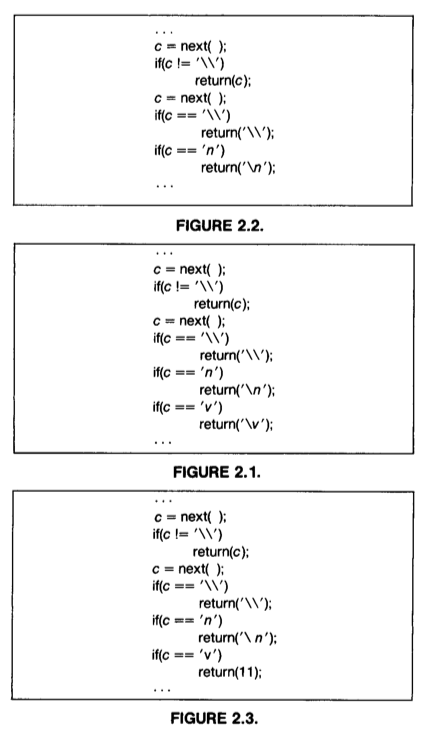
\includegraphics[width=0.8\linewidth]{img/image_2023-01-13-05-03-27.png}
    \caption{Teaching a compiler what the "\textbackslash v" sequence is. We may add a statement to return the ascii encoding of \textbackslash v (11), compile the compiler, and then use it to compile a program that knows what \textbackslash v is. }. We may then alter the source to be like Figure 2.3 without any mention of \textbackslash v but still compile programs with \textbackslash v just fine.
\end{figure}

\begin{figure}[H]
    \centering
    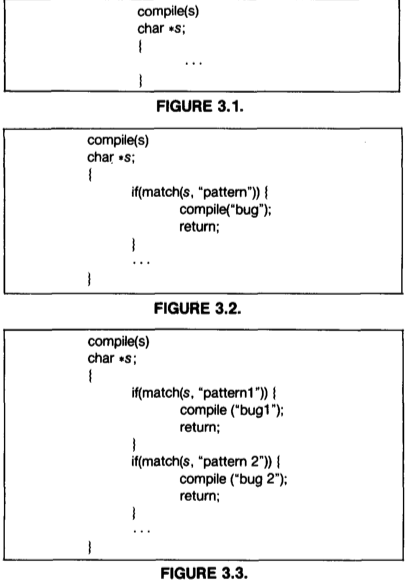
\includegraphics[width=0.8\linewidth]{img/image_2023-01-13-05-08-29.png}
\end{figure}

Next, consider the above scenario where we insert a login Trojan to insert backdoors into code matching the unix login function. We may then compile the $ c $ compiler to do just that, and then change the source to what it should look like without the Trojan. Compiling the compiler one more time will now produce a compiler binary that looks completely innocent but will reinsert the Trojan wherever it can.


The moral of the story is that you can't trust code that you didn't totally create yourself. But it's awfully difficult to use only code written by oneself. So take security seriously.


\end{document}
